\documentclass[12pt]{article}
 
\newenvironment{sol}[1][Solution]{\begin{trivlist}\item[\hskip\labelsep {\bfseries #1:}]}{\end{trivlist}}
\usepackage{minted}
%\usemintedstyle{perldoc}
\usemintedstyle{vs}
\usepackage{graphicx}
\graphicspath{./}
\usepackage{diagbox}
\usepackage[margin=1in]{geometry} 
\usepackage{amsmath,amsthm,amssymb}
\usepackage{times,url}

\begin{document}
\renewcommand{\qedsymbol}{\filledbox}
\begin{flushleft}
Homework 3: \ \ \ \
Name \underline{ \ \ \ \ \  Bingying Liang \ \ \ \ \ \ \ \  } \ \ \ \ 
ID \underline{ \ \  \ \ \ \ \ \ 48999397 \ \ \ \ \ \ \ }
\end{flushleft}
\begin{enumerate}
    \item \ [15 pts] Given you have three dice where die D1 has faces $\{0, 2, 2, 2, 3, 3\}$ die D2 has faces $\{2,3,3,5\}$ and Die D3 has faces $\{2,2,2, 1,1,1, 0, 0 \}$. Fill in the dynamic programming table for D1 and D2 and D3.
    \begin{enumerate}
        \item[(i)]  Indicate how many different ways you can roll the value 7 using all the three dice in the problem.
        \begin{sol}
            45
        \end{sol}
        \item[(ii)] Indicate how many different ways you can roll the value 11 using all three dice in the problem.
        \begin{sol}
            0. Because Max face of D1, D2, D3 are 3,5,2 and then $3 + 5+2 = 10 < 11$.
        \end{sol}
        \item[(iii)] What is the Probability of rolling a 7?
        \begin{sol}
        \begin{align*}
            \frac{42}{6\times 4\times8} =\frac{42}{192}=\frac{7}{32}
        \end{align*}
        \end{sol}

    \end{enumerate}
    \begin{center}
        \begin{tabular}{|c|c|c|c|}
        \hline
            die  &  D1 & D1+D2 & D1+D2+D3 \\
            sum    & (ways)&(ways) &(ways) \\
            \hline
            0 & 1 & 0 & 0\\
            \hline
            1  & 0 & 0& 0\\
            \hline
            2  & 3 & 1& 2\\
            \hline
            3  & 2& 2& 7\\
            \hline
            4  & 0& 3& 15\\
            \hline
            5  & 0& 9& 33\\
            \hline
            6  & 0& 4& 44\\
            \hline
            7  & 0& 3& 45\\
            \hline
            8  & 0& 2& 25\\
            \hline
            9  & 0& 0& 15\\
            \hline
            10  &0 & 0& 6\\
            \hline
            11 & 0 & 0 & 0\\
            \hline
            Sum ways & 6 & 24 & 192 \\ 
            \hline
            
            
        \end{tabular}
    \end{center}
    \item \ [15 pts] You have 4 items to consider:
    \begin{itemize}
        \item Item 1 weighs 1 lb and is worth \$2.
        \item Item 2 weighs 5 lbs and is worth \$7.
        \item Item 3 weighs 6 lbs and is worth \$8.
        \item Item 4 weighs 2 lbs and is worth \$3.
    \end{itemize}
    \begin{enumerate}
        \item[(i)] If you can carry 11 lbs and can not divide the items. There is also only one of each item available. Set up the table to show which items you would take.
        \begin{sol}
                   \hspace*{\fill}
            \begin{center}
                \begin{tabular}{|c|c|c|c|c|}
                \hline
                     Carry & Value from  & Value from & Value from & Value from \\
                weight & item 1 & item 1 and 2 & item 1 to 3 & item 1 to 4\\
                \hline
                0 & 0 &0 &0 &0 \\
                \hline
                1 & 2 &2 &2 &2 \\
                \hline
                2 &2 & 2& 2& 3 \\
                \hline
               3 &2 & 2& 2& 5\\
                 \hline
               4&2 &2 & 2& 5\\
                 \hline
               5 &2 &7 &7 & 7 \\
                 \hline
               6 &2 &9 &9& 9\\
                 \hline
               7 &2 &9 &10 & 10\\
                 \hline
               8 &2 &9 & 10& 12\\
                 \hline
               9 &2 &9 & 10& 13\\
                 \hline
               10 &2 &9 & 10& 13\\
                     \hline
               11 &2 &9 & 15& 15\\
                     \hline
               12 &2 &9 & 17& 17\\
                     \hline
               13 &2 &9 & 17& 18\\
                     \hline
               14 &2 &9 & 17& 20 \\
               \hline
                \end{tabular}
            \end{center}
            Therefore, if I can carry 11 lbs, I will take item2, item3 and the value of them is \$15.
        \end{sol}
        \item[(ii)] Assume you can divide the items. That is 25\% of an item weighs 25\% as much and is worth 25\% of the value. You can take a maximum of 100\% of an item. That is there is only one of each item available. Which items would you take and how much of each item would you take?
        \begin{sol}
        \hspace*{\fill}
        \begin{center}
            \begin{tabular}{|c|c|c|c|c|}
            \hline
                Item &  1 &  2& 3  & 4\\
                \hline
                Weight  & 1 & 5  & 6 & 2 \\
                \hline
                Worth & 2 & 7 & 8 & 3\\
                \hline
                Ratio $(\frac{Worth}{Weight})$ & 2 & 1.4 & $\frac{8}{6}$ & 1.5 \\
                \hline
            \end{tabular}
                \begin{tabular}{|c|c|c|c|c|}
                \hline
                     Carry & Value from  & Value from & Value from & Value from \\
                weight & item 1 & item 1 and 4 & item 1, 4, 2 & item 1, 4, 2, 3 \\
                \hline
                0 & 0 &0 &0 &0 \\
                \hline
                1 & 2 &2 &2 &2 \\
                \hline
                2 &2 & 3.5& 3.5& 3.5 \\
                \hline
               3 &2 & 5& 5& 5\\
                 \hline
               4&2 &5 & 6.4& 6.4\\
                 \hline
               5 &2 &5 &7.8& 7.8 \\
                 \hline
               6 &2 &5 &9.2& 9.2\\
                 \hline
               7 &2 &5 &10.6 & 10.6\\
                 \hline
               8 &2 &5 & 12& 12\\
                 \hline
               9 &2 &5 & 12& $\frac{40}{3}\approx 13.33$\\
                 \hline
               10 &2 &5 & 12& $\frac{44}{3} \approx 14.67$\\
                     \hline
               11 &2 &5 & 12& 16\\
                     \hline
               12 &2 &5 & 12& $\frac{52}{3} \approx 17.33$\\
                     \hline
               13 &2 &5 & 12& $\frac{56}{3} \approx 18.67$\\
                     \hline
               14 &2 &5 & 12& 20 \\
               \hline
                \end{tabular}
        \end{center}       
        According to the ratio, I take the item 1 first, then item 4, then item 2, then item 3
        Therefore, if I can carry 11 lbs, I will take  100\% item1, 100\% item4, 100\% item2,  50\% item3 and the value of them is $\$16$.
        \end{sol}
    \end{enumerate}


    \item \ [10 pts] A table was created and filled in for determining the Longest Increasing Subsequence. The final row of the table is shown below.
    \begin{center}
            \begin{tabular}{|c|c|c|c|c|c|}
    \hline
         1&2 & 4 & 5 & 6 & 8  \\
    \hline
    \end{tabular}
    \end{center}
    \begin{enumerate}
        \item [(i)] What does the value 6 indicate?
        \begin{sol}
            The 5th value of the longest Increasing subsequence is 6. 
        \end{sol}
        \item [(i)] What does the value 5 indicate?
        \begin{sol}
            The 4th value of the longest Increasing subsequence is 5.
        \end{sol}
        \item [(i)] How long is the Longest Increasing Subsequence?
           \begin{sol}
        6
    \end{sol}
    \end{enumerate}
 

    \item \ [10 pts] Set up a table and show the Longest Common Subsequence for the following two strings:
    \begin{align*}
        \text{A \ A \ C \ C \ T \ C \ G \ T \ A \ C and \ A \ C \ C \ A \ T \ G \ G \ T \ A \ A \ C \ T}
    \end{align*}
    (You may do this in Excel and show your results here)
    \begin{sol}
    \hspace*{\fill}
    \begin{center}
        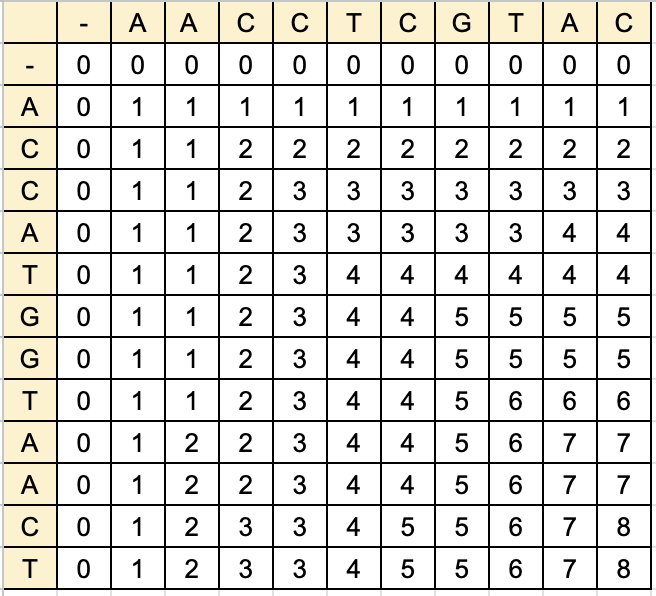
\includegraphics[width=0.6\textwidth]{p1.png}
    \end{center}
    \end{sol}
     The longest Common Subsequence is ``ACCTGTAC" and its length is 8.

    \item \ [10 pts] Show the table to find the Levensthein Edit Distance of the following two strings: What is the edit distance?
        \begin{align*}
        \text{A \ C \ T \ G \ T \ A \ C \ G \ C and \ A \ T \ X \ T \ C \ G \ C \ Y \ M}
    \end{align*}
    (You may do this in Excel and show your results here)
    \begin{sol}
        \hspace*{\fill}
            \begin{center}
        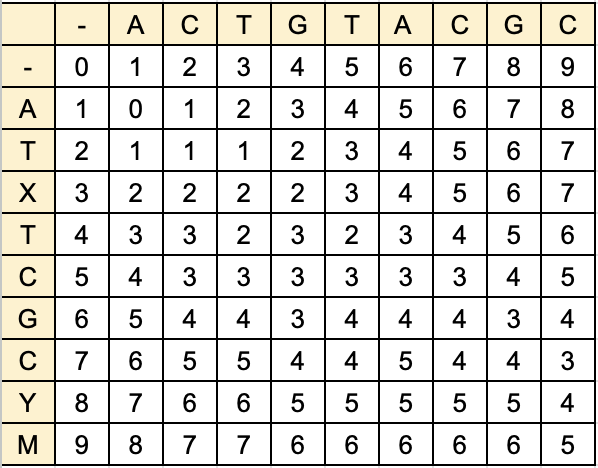
\includegraphics[width=0.5\textwidth]{p2.png}
    \end{center}
    ACTGTACGC $\rightarrow$ ATGTACGC (delete ``C")\\
    ATGTACGC $\rightarrow$ ATXTACGC (replace ``G" with ``X")\\
    ATXTACGC $\rightarrow$ ATXTCGC (delete ``A")\\
    ATXTCGC $\rightarrow$ ATXTCGCY (insert ``Y")\\
    ATXTCGCY $\rightarrow$ ATXTCGCYM (insert ``M")\\
     
    \end{sol}


    \item \ [10 pts] Consider two strings. The length of the first string is unknown and the length of the second string is fifteen. The Levensthein edit distance between the strings is 6.
    \begin{enumerate}
        \item [a.] What is the maximum possible length of the first string?
        \begin{sol}
        21
        \end{sol}
        \item [b.] What is the minimum possible length of the first string?
        \begin{sol}
        9
        \end{sol}
        \item [c.] What is the maximum possible length of the Longest Common Subsequence of the two strings?
        \begin{sol}
            15
        \end{sol}
        \item [d.] What is the minimum possible length of the Longest Common Subsequence of the two strings?
        \begin{sol}
            9
        \end{sol}
        
    \end{enumerate}
    
    \item \ [10 pts] Set up the table for the Extended Euclidian Algorithm and use it to find
    \begin{align*}
        1/19 \text{ modulo } 3315
    \end{align*}
    \begin{sol}
    \hspace*{\fill}
    \begin{center}
        \begin{tabular}{|c|c|c|c|c|c|c|}
        \hline
          & A & B & Q & R & $\alpha$ & $\beta$ \\
          \hline
        -1&   &   &   &   & 1 & 0\\   
        \hline
               0&   3315 &  19 & 174  &  9 &  0 & 1 \\   
        \hline
               1& 19  & 9  &  2 &  1 & 1 & -174\\   
        \hline
               2& 9  &  1 &  9 &   0 & -2 & 349\\   
        \hline
               3&  1 &  0 &  - & -  &  19& 3315 \\   
        \hline

        \end{tabular}
    \end{center}
    \begin{align*}
        &-2 \times 3315 + 19 \times 349 = 1\\
        &(-2 \times 3315) \ \% \ 3315 + (19 \times 349)\ \% \ 3315 = 1 \ \% \ 3315\\
        & 0 + (19 \times 349) \ \% \ 3315 = 1\\
        & \therefore (19 \times 349) \ \% \ 3315 = 1\\
        & (19 \times \frac{1}{19}) \ \% \ 3315 = 1\\
        & \therefore \frac{1}{19} \ \% \ 3315 = 349
    \end{align*}
    \end{sol}

    \item \ [20 pts] Bob encoded a message to Alice using RSA. Alice’s public key is $e = 82313$ with a modulus of $467807$. Using a quantum computer, you were able to factor the modulus into the product of two primes, $677 * 691$. Assumes the cipher text is 2.
    \begin{enumerate}
        \item [a.] What is Alice’s Private Key (show your table for calculating the Extended Euclidian Algorithm)
        \begin{sol}
            \begin{align*}
                &n = 467807 = (pq) = 677 \times 691 \\
                &\phi(n) = (p-1)(q-1) = 676 \times 690 = 466440\\
                &d = \frac{1}{e} \ \% \ \phi(n) =\frac{1}{82313} \ \% \ 466440 \\
            \end{align*}
            \begin{center}

    \begin{tabular}{|c|c|c|c|c|c|c|}
        \hline
                 & A   & B        & Q      & R   & $\alpha$ & $\beta$ \\
          \hline
            -1  &     &           &        &     &    1& 0\\   
        \hline
               0& 466440 &  82313 & 5  &  54875 &  0  & 1 \\   
        \hline
               1& 82313  & 54875  &  1 &  27438  & 1 & -5 \\   
        \hline
               2& 54875  &  27438 &  1 &   27437 & -1 & 6\\   
        \hline
               3& 27438 &  27437 &  1 &  1  &  2 & -11  \\  
        \hline
               4& 27437 & 1 &  27437 &    0    &  -3 & 17    \\
        \hline
               5 & 1 & 0  & - & - & 82313 &  -466440\\
        \hline
        \end{tabular}
        \begin{align*}
            & -3 \times 466440 + 17 \times 82313  = 1 \\
            & (-3 \times 466440) \ \% 466440 \ + (17 \times 82313) \ \% \ 466440= 1 \ \% \ (466440) \\
            & 0 + (17 \times 82313) \ \% \ 466440 = 1 \\ 
            & \therefore (17 \times 82313) \ \% \ 466440 = 1 \\
            & \because (\frac{1}{82313} \times 82313) \ \% \ 466440 = 1 \\
            & \therefore(\frac{1}{82313}) \ \% \ 466440 = 17 \\ 
            & \therefore d = 6\\
            & \therefore \text{Alice's Private Key is } \{ 17, 467807 \}
        \end{align*}
            \end{center}
        \end{sol}
        \item [b.] What was the un-encrypted message Bob was sending to Alice?
        \begin{sol}
        \begin{align*}
            & \because c = 2 \\
            & \therefore 2^{17} \ \% \ 466440 = 131072 \\
            & \therefore 131072 \text{ is the un-encrypted message Bob was sending to Alice. }
        \end{align*}
        \end{sol}
    \end{enumerate}
\end{enumerate}
\end{document}
